% =============================================================================
% Kapitel 2: Grundlagen
% -----------------------------------------------------------------------------
% Was hinein gehört (Richtwert 12--18 Seiten):
%  2.1 Röntgen-Nahfeldholographie (NFH)
%      - Synchrotronstrahlung, Kohärenz, Phasenkontrast
%      - komplexer Brechungsindex n = 1 - delta + i beta, Projektionsnäherung,
%        Exit-Wave psi = exp(iO) * P (Notation der Aufgabenstellung)
%      - Kegelstrahl-Geometrie an P05: Quelle -> Objekt (z01) -> Detektor (z02)
%  2.2 Fresnel-Propagation
%      - Fresnel-Kirchhoff/paraxiale Näherung, Propagator D_Fr im Fourierraum
%      - Intensität I = |D_Fr(psi)|^2, Verlust der Phase
%  2.3 Fresnel-Zahl und Fresnel-Skalierungstheorem
%      - Definition Fr (pixelbezogen), effektive Distanz z_eff, Vergrößerung M
%      - Sensitivität des Hologramms gegenüber Fr (-> warum Autofokus möglich ist)
%  2.4 Phase Retrieval
%      - Klassiker: Fienup 1982 (iterative Projektionen), Paganin 2002 (TIE, ein
%        Abstand, homogenes Objekt), CTF-Methoden
%      - ASRM (Dora et al. 2024): Modell, Regularisierung, Lösung ohne Support
%  2.5 Das Autofokus-Problem
%      - Fr als freier Modellparameter; Fehlfokus -> Artefakte
%      - modellbasierter Autofokus (Dora et al. 2025): Zielfunktion, Optimierer
%        (z. B. Nelder-Mead), Laufzeit -> Motivation für Lernverfahren
%  2.6 Deep Learning für Regression
%      - CNN-Bausteine, Verlustfunktionen (MSE/MAE/Huber), Normierung der Ziel-
%        größe (Fr vs. log Fr vs. z01), Generalisierung, Datenaugmentierung
%  2.7 Simulationsbasierte Inferenz (SBI)
%      - Idee: Simulator + neuronaler Dichteschätzer -> Posterior p(Fr | I)
%      - NPE/NLE/NRE, sbi-Toolkit (Tejero-Cantero 2020, Boelts 2025),
%        Praxisleitfaden (Deistler 2025); Nutzen: Unsicherheit statt Punktschätzung
% Konventionen: Notation aus main.tex (\Fr, \zOne, \zTwo, \magn, \wl, \dx, \prop)
% =============================================================================
\chapter{\lang{Grundlagen}{Fundamentals}}
\label{ch:grundlagen}

\section{\lang{Röntgen-Nahfeldholographie}{X-ray Near-field Holography}}
\label{sec:grundlagen:nfh}

\lang{%
Ein Objekt wird durch seinen komplexen Brechungsindex
$n(\vect{r}) = 1 - \delta(\vect{r}) + \mathrm{i}\beta(\vect{r})$ beschrieben, wobei
$\delta$ die Phasenverschiebung und $\beta$ die Absorption kodiert. In
Projektionsnäherung ergibt sich die Austrittswelle hinter dem Objekt als Produkt
aus Beleuchtung $P$ und Objekttransmission.
}{%
An object is described by its complex refractive index
$n(\vect{r}) = 1 - \delta(\vect{r}) + \mathrm{i}\beta(\vect{r})$, where $\delta$
encodes the phase shift and $\beta$ the absorption. In the projection
approximation the exit wave behind the object is the product of the illumination
$P$ and the object transmission.
}
\todo{\lang{Herleitung und Skizze der Geometrie ergänzen.}{Add derivation and a sketch of the geometry.}}

\section{\lang{Fresnel-Propagation}{Fresnel Propagation}}
\label{sec:grundlagen:propagation}

% Beispiel: nummerierte Gleichung mit Label und Verweis
\lang{Die Intensität in der Detektorebene ergibt sich durch Fresnel-Propagation der Austrittswelle $\psi$:}%
{The intensity in the detector plane follows from Fresnel propagation of the exit wave $\psi$:}
\begin{equation}
  I = \abs{\prop{\Fr}(\psi)}^2,
  \qquad
  \prop{\Fr}(\psi) = \mathcal{F}^{-1}\!\left[\exp\!\left(-\mathrm{i}\pi\,\frac{\xi^2+\eta^2}{\Fr}\right)\mathcal{F}[\psi]\right],
  \label{eq:grundlagen:propagation}
\end{equation}
\lang{%
wobei $\mathcal{F}$ die zweidimensionale Fourier-Transformation und $(\xi,\eta)$
die auf die Pixelgröße normierten Ortsfrequenzen bezeichnen. Die Phase von
$\prop{\Fr}(\psi)$ geht bei der Messung verloren; ihre Rekonstruktion ist das
\ac{pr}-Problem \cite{fienup1982phase}.
}{%
where $\mathcal{F}$ denotes the two-dimensional Fourier transform and $(\xi,\eta)$
the spatial frequencies normalised to the pixel size. The phase of
$\prop{\Fr}(\psi)$ is lost in the measurement; recovering it is the \ac{pr}
problem \cite{fienup1982phase}.
}
\todo{\lang{Normierungskonvention mit HoloWizard abgleichen.}{Check normalisation convention against HoloWizard.}}

\section{\lang{Fresnel-Zahl und Fresnel-Skalierungstheorem}{Fresnel Number and Fresnel Scaling Theorem}}
\label{sec:grundlagen:fresnelzahl}

\lang{%
In der Kegelstrahlgeometrie mit Quelle--Objekt-Abstand $\zOne$ und
Quelle--Detektor-Abstand $\zTwo$ wirkt die geometrische Vergrößerung
$\magn = \zTwo/\zOne$. Nach dem Fresnel-Skalierungstheorem ist die Aufnahme
äquivalent zu einer Parallelstrahl-Propagation über die effektive Distanz
$\zEff = (\zTwo - \zOne)/\magn$ mit effektiver Pixelgröße $\dx/\magn$. Die
pixelbezogene Fresnel-Zahl lautet damit
}{%
In the cone-beam geometry with source--object distance $\zOne$ and
source--detector distance $\zTwo$ the geometric magnification is
$\magn = \zTwo/\zOne$. By the Fresnel scaling theorem the acquisition is
equivalent to a parallel-beam propagation over the effective distance
$\zEff = (\zTwo - \zOne)/\magn$ with effective pixel size $\dx/\magn$. The
pixel-based Fresnel number therefore reads
}
\begin{equation}
  \Fr = \frac{\dx^2}{\wl\,(\zTwo - \zOne)\,\magn},
  \qquad \magn = \frac{\zTwo}{\zOne},
  \label{eq:grundlagen:fresnelzahl}
\end{equation}
\lang{%
mit der Wellenlänge $\wl$ und der Detektorpixelgröße $\dx$. Bei festem $\zTwo$
hängt $\Fr$ nur noch von $\zOne$ ab, sodass Autofokus wahlweise als Schätzung von
$\Fr$ oder von $\zOne$ formuliert werden kann (\cref{fig:grundlagen:fresnelzahl}).
}{%
with wavelength $\wl$ and detector pixel size $\dx$. For fixed $\zTwo$, $\Fr$
depends on $\zOne$ only, so autofocus can equivalently be posed as estimating
$\Fr$ or $\zOne$ (\cref{fig:grundlagen:fresnelzahl}).
}

% Beispiel: Abbildung -- Snippet wurde mit tools/export_figures.py erzeugt und
% enthält Quelle (Run, Commit) als Kommentar. Caption dort anpassen.
% ---------------------------------------------------------------------------
% Automatisch erzeugt von tools/export_figures.py -- Quelle der Abbildung:
%   Run:     (Beispiel) Skript-Erzeugung mit thesis/thesis.mplstyle, kein Trainingslauf;
%            Formel: Fr = dx^2 / (lambda (z02 - z01) M), M = z02/z01
%   Commit:  3579d3497f59dc80f80f967b6bd080ae140fb157  (Working Tree hatte uncommittete Änderungen!)
%   Datum:   2026-10-01
%   Dateien: fresnelzahl.pdf
% Caption und ggf. Breite anpassen; diese Datei wird bei erneutem Export NICHT
% überschrieben (außer mit --force). Einbinden im Kapitel:
%   % ---------------------------------------------------------------------------
% Automatisch erzeugt von tools/export_figures.py -- Quelle der Abbildung:
%   Run:     (Beispiel) Skript-Erzeugung mit thesis/thesis.mplstyle, kein Trainingslauf;
%            Formel: Fr = dx^2 / (lambda (z02 - z01) M), M = z02/z01
%   Commit:  3579d3497f59dc80f80f967b6bd080ae140fb157  (Working Tree hatte uncommittete Änderungen!)
%   Datum:   2026-10-01
%   Dateien: fresnelzahl.pdf
% Caption und ggf. Breite anpassen; diese Datei wird bei erneutem Export NICHT
% überschrieben (außer mit --force). Einbinden im Kapitel:
%   % ---------------------------------------------------------------------------
% Automatisch erzeugt von tools/export_figures.py -- Quelle der Abbildung:
%   Run:     (Beispiel) Skript-Erzeugung mit thesis/thesis.mplstyle, kein Trainingslauf;
%            Formel: Fr = dx^2 / (lambda (z02 - z01) M), M = z02/z01
%   Commit:  3579d3497f59dc80f80f967b6bd080ae140fb157  (Working Tree hatte uncommittete Änderungen!)
%   Datum:   2026-10-01
%   Dateien: fresnelzahl.pdf
% Caption und ggf. Breite anpassen; diese Datei wird bei erneutem Export NICHT
% überschrieben (außer mit --force). Einbinden im Kapitel:
%   \input{figures/grundlagen/fresnelzahl}
% ---------------------------------------------------------------------------
\begin{figure}[htbp]
  \centering
  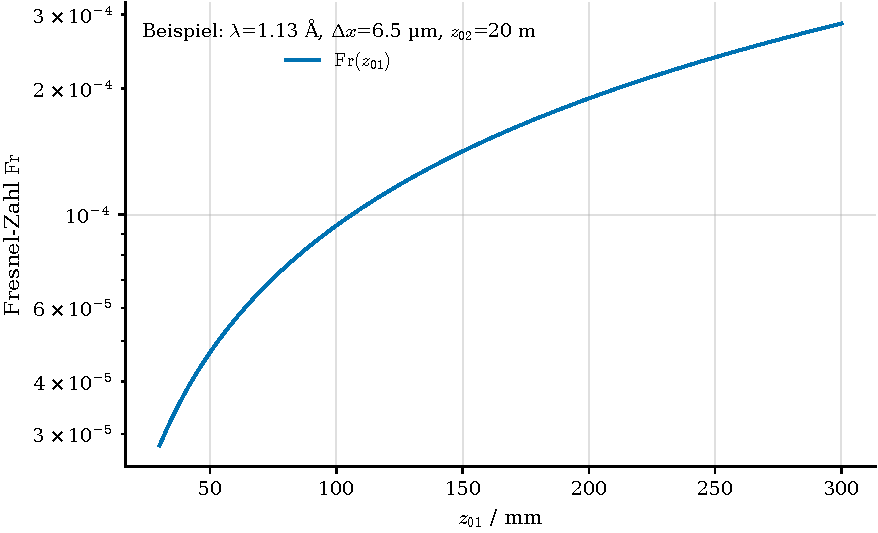
\includegraphics[width=0.8\textwidth]{figures/grundlagen/fresnelzahl}
  \caption[\lang{Fresnel-Zahl als Funktion des Abstands $\zOne$}{Fresnel number as a function of the distance $\zOne$}]{%
    \lang{Fresnel-Zahl $\Fr$ nach \cref{eq:grundlagen:fresnelzahl} als Funktion des
    Quelle--Objekt-Abstands $\zOne$ für Parameter in der Größenordnung des
    P05-Aufbaus ($\wl = \qty{1.13}{\angstrom}$ bzw.\ \qty{11}{\kilo\electronvolt},
    $\dx = \qty{6.5}{\micro\metre}$, $\zTwo = \qty{20}{\metre}$;
    vgl.\ \cite{dora2025autofocus}). Beispielabbildung im Stil
    \texttt{thesis.mplstyle}; durch eine echte Abbildung ersetzen.}%
    {Fresnel number $\Fr$ according to \cref{eq:grundlagen:fresnelzahl} as a
    function of the source--object distance $\zOne$ for parameters of the order
    of the P05 setup ($\wl = \qty{1.13}{\angstrom}$, i.e.\ \qty{11}{\kilo\electronvolt},
    $\dx = \qty{6.5}{\micro\metre}$, $\zTwo = \qty{20}{\metre}$;
    cf.\ \cite{dora2025autofocus}). Example figure in the
    \texttt{thesis.mplstyle} style; replace with a real figure.}}
  \label{fig:grundlagen:fresnelzahl}
\end{figure}

% ---------------------------------------------------------------------------
\begin{figure}[htbp]
  \centering
  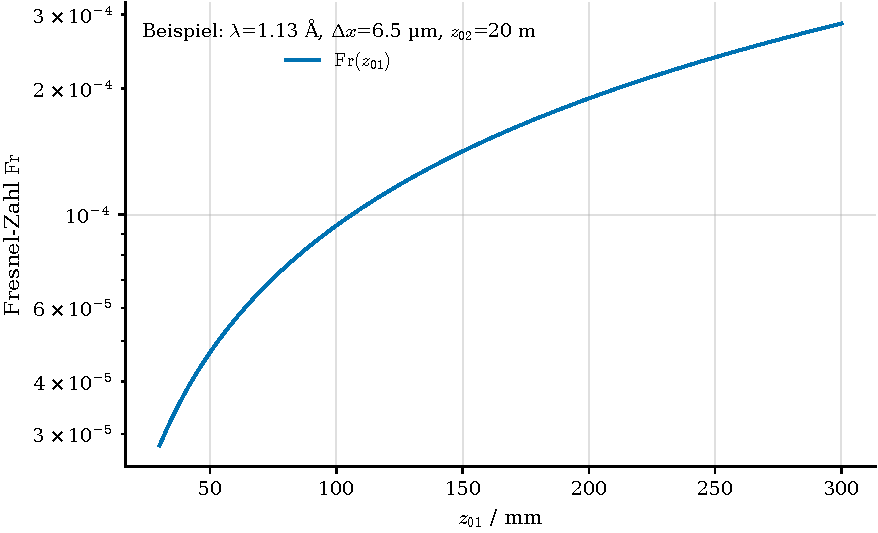
\includegraphics[width=0.8\textwidth]{figures/grundlagen/fresnelzahl}
  \caption[\lang{Fresnel-Zahl als Funktion des Abstands $\zOne$}{Fresnel number as a function of the distance $\zOne$}]{%
    \lang{Fresnel-Zahl $\Fr$ nach \cref{eq:grundlagen:fresnelzahl} als Funktion des
    Quelle--Objekt-Abstands $\zOne$ für Parameter in der Größenordnung des
    P05-Aufbaus ($\wl = \qty{1.13}{\angstrom}$ bzw.\ \qty{11}{\kilo\electronvolt},
    $\dx = \qty{6.5}{\micro\metre}$, $\zTwo = \qty{20}{\metre}$;
    vgl.\ \cite{dora2025autofocus}). Beispielabbildung im Stil
    \texttt{thesis.mplstyle}; durch eine echte Abbildung ersetzen.}%
    {Fresnel number $\Fr$ according to \cref{eq:grundlagen:fresnelzahl} as a
    function of the source--object distance $\zOne$ for parameters of the order
    of the P05 setup ($\wl = \qty{1.13}{\angstrom}$, i.e.\ \qty{11}{\kilo\electronvolt},
    $\dx = \qty{6.5}{\micro\metre}$, $\zTwo = \qty{20}{\metre}$;
    cf.\ \cite{dora2025autofocus}). Example figure in the
    \texttt{thesis.mplstyle} style; replace with a real figure.}}
  \label{fig:grundlagen:fresnelzahl}
\end{figure}

% ---------------------------------------------------------------------------
\begin{figure}[htbp]
  \centering
  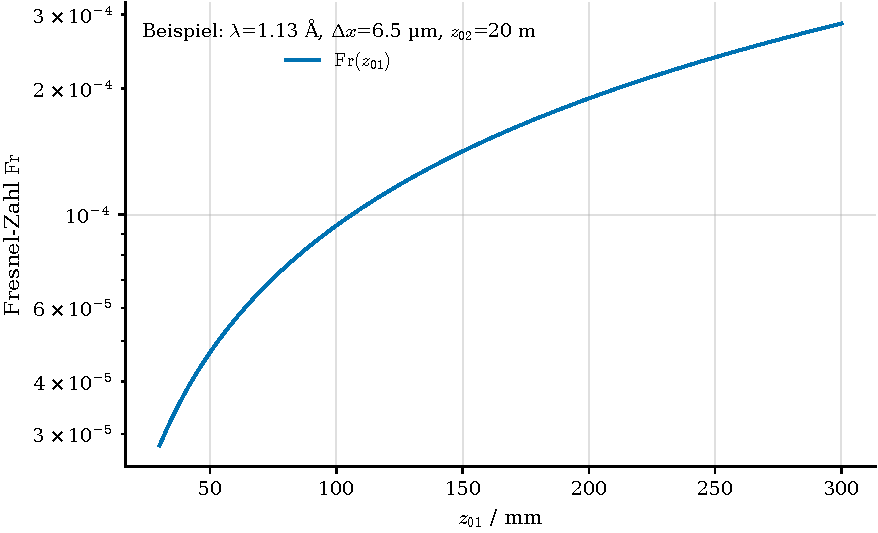
\includegraphics[width=0.8\textwidth]{figures/grundlagen/fresnelzahl}
  \caption[\lang{Fresnel-Zahl als Funktion des Abstands $\zOne$}{Fresnel number as a function of the distance $\zOne$}]{%
    \lang{Fresnel-Zahl $\Fr$ nach \cref{eq:grundlagen:fresnelzahl} als Funktion des
    Quelle--Objekt-Abstands $\zOne$ für Parameter in der Größenordnung des
    P05-Aufbaus ($\wl = \qty{1.13}{\angstrom}$ bzw.\ \qty{11}{\kilo\electronvolt},
    $\dx = \qty{6.5}{\micro\metre}$, $\zTwo = \qty{20}{\metre}$;
    vgl.\ \cite{dora2025autofocus}). Beispielabbildung im Stil
    \texttt{thesis.mplstyle}; durch eine echte Abbildung ersetzen.}%
    {Fresnel number $\Fr$ according to \cref{eq:grundlagen:fresnelzahl} as a
    function of the source--object distance $\zOne$ for parameters of the order
    of the P05 setup ($\wl = \qty{1.13}{\angstrom}$, i.e.\ \qty{11}{\kilo\electronvolt},
    $\dx = \qty{6.5}{\micro\metre}$, $\zTwo = \qty{20}{\metre}$;
    cf.\ \cite{dora2025autofocus}). Example figure in the
    \texttt{thesis.mplstyle} style; replace with a real figure.}}
  \label{fig:grundlagen:fresnelzahl}
\end{figure}


\section{Phase Retrieval}
\label{sec:grundlagen:pr}
\todo{\lang{Fienup \cite{fienup1982phase}, Paganin \cite{paganin2002phase}, CTF, ASRM \cite{dora2024asrm}.}{Fienup \cite{fienup1982phase}, Paganin \cite{paganin2002phase}, CTF, ASRM \cite{dora2024asrm}.}}

\section{\lang{Das Autofokus-Problem}{The Autofocus Problem}}
\label{sec:grundlagen:autofokus}
\todo{\lang{Modellbasierter Autofokus nach \cite{dora2025autofocus}: Zielfunktion, Optimierer, Laufzeit.}{Model-based autofocus following \cite{dora2025autofocus}: objective, optimiser, runtime.}}

\section{\lang{Deep Learning für Regressionsaufgaben}{Deep Learning for Regression}}
\label{sec:grundlagen:dl}
\todo{\lang{CNN-Bausteine, Verlustfunktionen, Zielgrößen-Normierung; Software: PyTorch \cite{paszke2019pytorch}.}{CNN building blocks, loss functions, target normalisation; software: PyTorch \cite{paszke2019pytorch}.}}

\section{\lang{Simulationsbasierte Inferenz}{Simulation-based Inference}}
\label{sec:grundlagen:sbi}
\todo{\lang{\ac{sbi}-Grundidee, \ac{npe}; Toolkit \cite{tejerocantero2020sbi,boelts2025sbireloaded}; Praxisleitfaden \cite{deistler2025sbi}.}{\Ac{sbi} basics, \ac{npe}; toolkit \cite{tejerocantero2020sbi,boelts2025sbireloaded}; practical guide \cite{deistler2025sbi}.}}
